\documentclass[12pt, twoside]{article}
\usepackage[francais]{babel}
\usepackage[T1]{fontenc}
\usepackage[latin1]{inputenc}
\usepackage[left=5mm, right=5mm, top=5mm, bottom=5mm]{geometry}
\usepackage{float}
\usepackage{graphicx}
\usepackage{array}
\usepackage{multirow}
\usepackage{amsmath,amssymb,mathrsfs}
\usepackage{textcomp}
\pagestyle{empty}
\usepackage{soul}
\usepackage{eurosym}


\begin{document} 



\begin{flushleft}
NOM PRENOM: \ldots \ldots \ldots \ldots \ldots \ldots \ldots \ldots \ldots
 \end{flushleft}


\begin{center}
{\fbox{$6^{e}\ldots$ \qquad \qquad \textbf{\Large{Devoir surveill� 5 }}
\qquad \qquad \ldots/03/2012}}
\end{center}


\bigskip
 

\textit{Les exercices 1, 2 et 4 sont � faire sur
la photocopie. Les autres sont � faire sur votre feuille pr�par�e.}

\bigskip


\ul{\textbf{Exercice 1:}} \textit{(3 points)}


\begin{tabular}{cc}
\begin{minipage}{7cm}
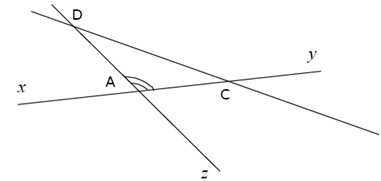
\includegraphics[width=7cm]{images/ex1.jpg}
\end{minipage}
&
\begin{minipage}{12cm}
\begin{enumerate}
  \item Nommer l'angle cod� sur la figure de deux fa�ons possibles:
  
  \ldots \ldots \ldots \ldots \ldots \ldots \ldots \ldots \ldots \ldots \ldots
  \ldots \ldots \ldots \ldots \ldots \ldots \ldots \ldots 
  \item Sur la figure, coder l'angle $\widehat{xCu}$.
  \item Compl�ter le tableau ci-dessous en mettant une croix:
  
  \enskip
  
  
  \begin{tabular}{|c|c|c|c|c|}
  \hline
  angles & aigu & obtus & plat & droit \\
  \hline
  $\widehat{xAz}$ & & & & \\
  \hline
  
  $\widehat{ADC}$ & & & & \\
  
  \hline
  
  $\widehat{DCu}$ & & & & \\
  
  \hline
  \end{tabular} 
\end{enumerate}
\end{minipage}
\end{tabular}

\bigskip

\ul{\textbf{Exercice 2:}} \textit{(4 points)}

\begin{enumerate}
  \item A l'aide du rapporteur, mesurer les angles suivants et �crire la
  r�ponse sur les pointill�s.
  
  \bigskip
  
  \bigskip
  
  \bigskip
  
  \bigskip
  
   \bigskip
  
  \bigskip
  
  \bigskip
  
  \bigskip    
  
  \bigskip
  
  \bigskip
  
  \bigskip
  
  \bigskip  
  
  \qquad \qquad \qquad \qquad \ldots \ldots \qquad \qquad \qquad \qquad \qquad
  \qquad \qquad \qquad \qquad \ldots \ldots
 \end{enumerate} 
  
  \bigskip
  
  \begin{tabular}{cc}
  \begin{minipage}{9cm}
  2. Tracer un angle $\widehat{BEL}$ de mesure 37�. 
  \end{minipage}
  &
  \begin{minipage}{9cm}
  3. Tracer un angle $\widehat{SIT}$ de mesure 124�.
  \end{minipage}
  \end{tabular}
  
   \bigskip
  
  \bigskip
  
   \bigskip
  
  \bigskip
  
  \bigskip
  
  \bigskip    
  
  \bigskip
  
  \bigskip
  
  \bigskip
  
  \bigskip  
  
  

 \bigskip
  
  \bigskip    
  
  \bigskip
  

  
\bigskip

\bigskip


\bigskip

\bigskip


\ul{\textbf{Exercice 3:}} \textit{(2,5 points)}


Les deux triangles ci-dessous sont trac�s � main lev�e. Construire ces deux
triangles en vraie grandeur.


  \bigskip    
  
  \bigskip
  
  \bigskip
  
  \bigskip
  
  
  \bigskip
  
  
  \bigskip 
  
  
 \ul{\textbf{Exercice 4:}} \textit{(2,5 points)}
 
 \begin{tabular}{cc}
 \begin{minipage}{9cm}
 1. Tracer la bissectrice [At) de l'angle $\widehat{DAF}$ 
 
 � l'aide du rapporteur.
 \end{minipage}
&
\begin{minipage}{9cm}
 \quad 2. Tracer la bissectrice [Bu) de l'angle $\widehat{FBE}$ 

\quad � l'aide du compas (vous laisserez vos traits de 

\quad construction).
\end{minipage}
 \end{tabular}

  \bigskip    
  
  \bigskip
  
  \bigskip
  
  \bigskip
  
  \bigskip 
  
   \bigskip
  
  \bigskip
  
  \bigskip 
  
    \bigskip 
  
  
    \bigskip
  
  \bigskip
  
  \bigskip 
  
    \bigskip
  
  \bigskip
  
  \bigskip 
  
    \bigskip 
  
  
    \bigskip
  
  \bigskip
  
  \bigskip 
  
   \ul{\textbf{Exercice 5:}} \textit{(3,5 points)}
   
   \enskip
   
   
    Chaque r�ponse doit �tre bien expliqu�e.
    
    
    \enskip
    
    
   \begin{tabular}{ccc}
   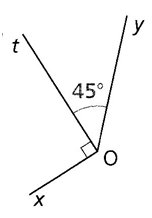
\includegraphics[width=2cm]{images/ex51.jpg} \qquad & \qquad 
   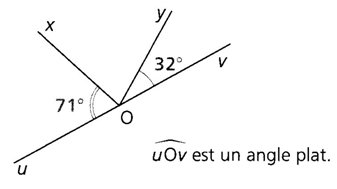
\includegraphics[width=5cm]{images/ex52.jpg} \qquad & \\
   
   
   \medskip
   
   
   \begin{minipage}{6cm}
   1. Calculer la mesure de 
   
   l'angle $\widehat{xOy}$.
   \end{minipage}

&

\begin{minipage}{6cm}
 2. Calculer la mesure de l'angle $\widehat{xOy}$.
\end{minipage}

&
\begin{minipage}{6cm}
 \qquad \quad 3. Les points G, H et I 
 
\qquad \quad sont-ils align�s? 
\end{minipage}
   \end{tabular}
  \\
   
  
   \bigskip 
  
  
 \ul{\textbf{Exercice 6:}} \textit{(4,5 points)}
 
 On sait que EFG est un triangle tel que EF=4cm, $\widehat{FEG}=110$� et EG=5cm.
 
 
 \begin{enumerate}
   \item Faire un sch�ma � main lev�e du triangle.
   \item Construire ce triangle en vraie grandeur.
   \item Placer un point H sur le segment [EF] tel que EH=3cm.
   \item Tracer la droite parall�le � la droite (FG) et passant par le point H.
   Cette droite coupe (EG) en J. Placer le point J.
   \item Construire la bissectrice de l'angle $\widehat{GEF}$. Cette
   bissectrice coupe la droite (JH) au point K. Placer le point K.
   \item Mesurer l'angle $\widehat{EKJ}$.
   
 \end{enumerate}  
  
  
  
 
   \bigskip 
  
  
 \ul{\textbf{Exercice BONUS}} \textit{(1,5 points)}  
 
 
\begin{tabular}{cc}
 \begin{minipage}{7cm}
   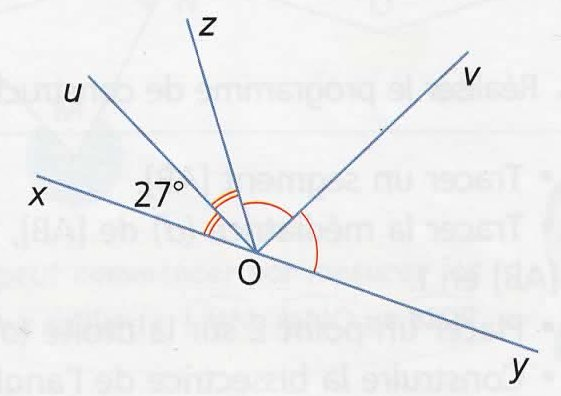
\includegraphics[width=6cm]{images/ex7.jpg}
 \end{minipage}
&
\begin{minipage}{11cm}
Sur la figure ci-contre:

$\bullet$ l'angle $\widehat{xOy}$ est plat,

$\bullet$ la demi-droite [Ou) est la bissectrice de l'angle $\widehat{xOz}$,

$\bullet$ la demi-droite [Ov) est la bissectrice de l'angle $\widehat{yOz}$.




\enskip

 \begin{enumerate}
  \item Calculer la mesure de l'angle $\widehat{zOy}$.
  \item L'angle $\widehat{uOv}$ est-il droit? Justifier votre r�ponse par un
  calcul.
\end{enumerate}

\end{minipage}
\end{tabular}

 
 


\end{document}
